\documentclass[10pt]{scrartcl}
\usepackage[english]{babel}
\usepackage{multirow}
\usepackage[default]{opensans}
\usepackage{sfmath} % sans font also for math
\usepackage[binary-units = true]{siunitx}
\usepackage{graphicx}
% defining the paper layout that no text overlaps with the header
\usepackage[
  top=35mm,
  headheight=25mm,
  headsep=3mm,
  bottom=30mm,
  left=25mm,
  right=25mm
]{geometry}

\usepackage[verbose]{placeins}
\usepackage{subcaption}
\usepackage{latexsym}
\usepackage[centertags]{amsmath}
\usepackage{amssymb}
\usepackage[]{glossaries}

\graphicspath{{figures/}}
% custom header and footpage
\usepackage{scrpage2}
\pagestyle{scrheadings} % you have to set the custom layout
% Head
%\chead{}
\ohead{
\includegraphics[height=25mm]{figures/EUCALL.png}}
% Foot
\ifoot{
\includegraphics[height=13.4mm]{figures/EU.png}} % left foot
\cfoot{%
  \begin{minipage}{100mm}%
    \begin{scriptsize}%
      \normalfont{This project has received funding from the}
      \textit{European Union’s Horizon 2020 research and innovation programme}
      \normalfont{under grant agreement No 654220.}
    \end{scriptsize}%
  \end{minipage}%
} % center foot
\ofoot{\thepage} % right foot

\usepackage{booktabs}

%%%%%%%%%%%%%%%%%%%%%%%%%%%%%%%%%%%%%%%%%%%%%%%
%   BIBLIOGRAPHY SETTINGS
\usepackage[bibstyle=nature,sorting=none,maxnames=1000,eprint=false,
defernumbers=true, backend=biber]{biblatex}
\usepackage{chemformula}
\usepackage{hyperref}


\renewcommand*\finalnamedelim{, and\addspace}
\DeclareNameAlias{sortname}{last-first}
\renewcommand{\newunitpunct}{, }

\AtEveryBibitem{%
  \clearfield{day}%
  \clearfield{month}%
  \clearfield{endday}%
  \clearfield{endmonth}%
  \clearfield{issn}%
  \clearfield{issue}%
}
%convert titles to hyperlinks using doi
\ExecuteBibliographyOptions{doi=true} \newbibmacro{string+doi}[1]{%
  \iffieldundef{doi}{#1}{\href{http://dx.doi.org/\thefield{doi}}{#1}}}
  \DeclareFieldFormat*{title}{\usebibmacro{string+doi}{\mkbibemph{#1}}}

\addbibresource{urls.bib}
\addbibresource{footnotes.bib}
\addbibresource{library.bib}

%%%%%%%%%%%%%%%%%%%%%%%%%%%%%%%%%%%%%%%%%%%%%%%
% GLOSSARY SETTINGS
\setacronymstyle{long-short}
\input{glossary}
\makeglossaries
%%%%%%%%%%%%%%%%%%%%%%%%%%%%%%%%%%%%%%%%%%%%%%%

% Zeilenabstand
\renewcommand{\baselinestretch}{1.2}


\usepackage{mathtools}
\DeclarePairedDelimiter\ceil{\lceil}{\rceil}
\DeclarePairedDelimiter\floor{\lfloor}{\rfloor}


\ihead{D4.4} % left head

\addbibresource{detector_sim_references.bib}

% sophisticated linking of references in the pdf and setting some options
\usepackage{url}                                                  % for correct typesettings of URLs
\usepackage{hyperref}                                             % for sophisticated linking of urls, dois, pictures, tables, etc.
\hypersetup{
    unicode=true,                                                 % non-Latin characters in Acrobat’s bookmarks
    pdftoolbar=true,                                              % show Acrobat’s toolbar?
    pdfmenubar=true,                                              % show Acrobat’s menu?
    pdffitwindow=false,                                           % window fit to page when opened
    pdfstartview={FitH},                                          % fits the width of the page to the window
    pdftitle={D4.4: Signal generation for plasma and non-plasma samples},                                        % title
    pdfauthor={C. Fortmann-Grote},                                           % author
    pdfsubject={EUCALL WP4 (SIMEX) Deliverable D4.4},                             % subject of the document
    pdfcreator={pdflatex},                                         % creator of the document
    pdfkeywords={EUCALL, SIMEX, scattering, diffraction, hot dense matter,
    single particle imaging, detector simulations},               % list of keywords
    pdfnewwindow=true,                                            % links in new PDF window
    colorlinks=true,                                              % false: boxed links; true: colored links
    linkcolor=blue,                                                % color of internal links (change box color with linkbordercolor)
    citecolor=blue,                                                % color of links to bibliography
    filecolor=blue,                                               % color of file links
    urlcolor=blue                                                 % color of external links
}

% Zeilenabstand
\renewcommand{\baselinestretch}{1.2}

\begin{document}
\makeatletter
\begin{titlepage}
\thispagestyle{scrheadings}
\begin{center}
$~$\\
\vspace{0cm}
{\Large\textbf{EUCALL}\\[2ex]
The European Cluster of Advanced Laser Light Sources}\\[4ex]
%
{\small\textbf{Grant Agreement number: 654220}}\\[8ex]
%
Work Package 4 -- SIMEX\\[4ex]
%
Deliverable D4.4\\
%
Simulated coherent scattering data from plasma and non--plasma samples\\[5ex]
%
Lead Beneficiary: HZDR, XFEL\\[5ex]
%
Carsten Fortmann-Grote, Jan-Philipp Burchert, Michael Bussmann,
  Marco Garten, Axel H\"ubl, Thomas Kluge,
  and Adrian P. Mancuso\\[4ex]
%
Due date: September 30, 2017\\
Delivery date: \today \\[4ex]
%
Project webpage: \url{www.eucall.eu}\\[6ex]
%
{%
\small
\begin{tabular}{|l|l|}
  \hline
  \multicolumn{2}{|l|}{ \textit{Deliverable Type} } \\
  \hline
  R = Report\hfill & R\\
  DEM = Demonstrator, pilot, prototype, plan designs & \\
  DEC = Websites, patents filing, press \& media actions, videos, etc. & \\
  OTHER = Software, technical diagram, etc. & \\
  \hline
  \multicolumn{2}{|l|}{\textit{Dissemination level}} \\
  \hline
  PU = Public, fully open, e.g. web & PU \\
  CO = Confidential, restricted under conditions set out in Model Grant
  Agreement\hspace*{17ex}\  & \\
  CI = Classified, information as referred to in Commission Decision 2001/844/EC
  & \\
  \hline
\end{tabular}
}

\end{center}
%
%\vfill
\centering{%
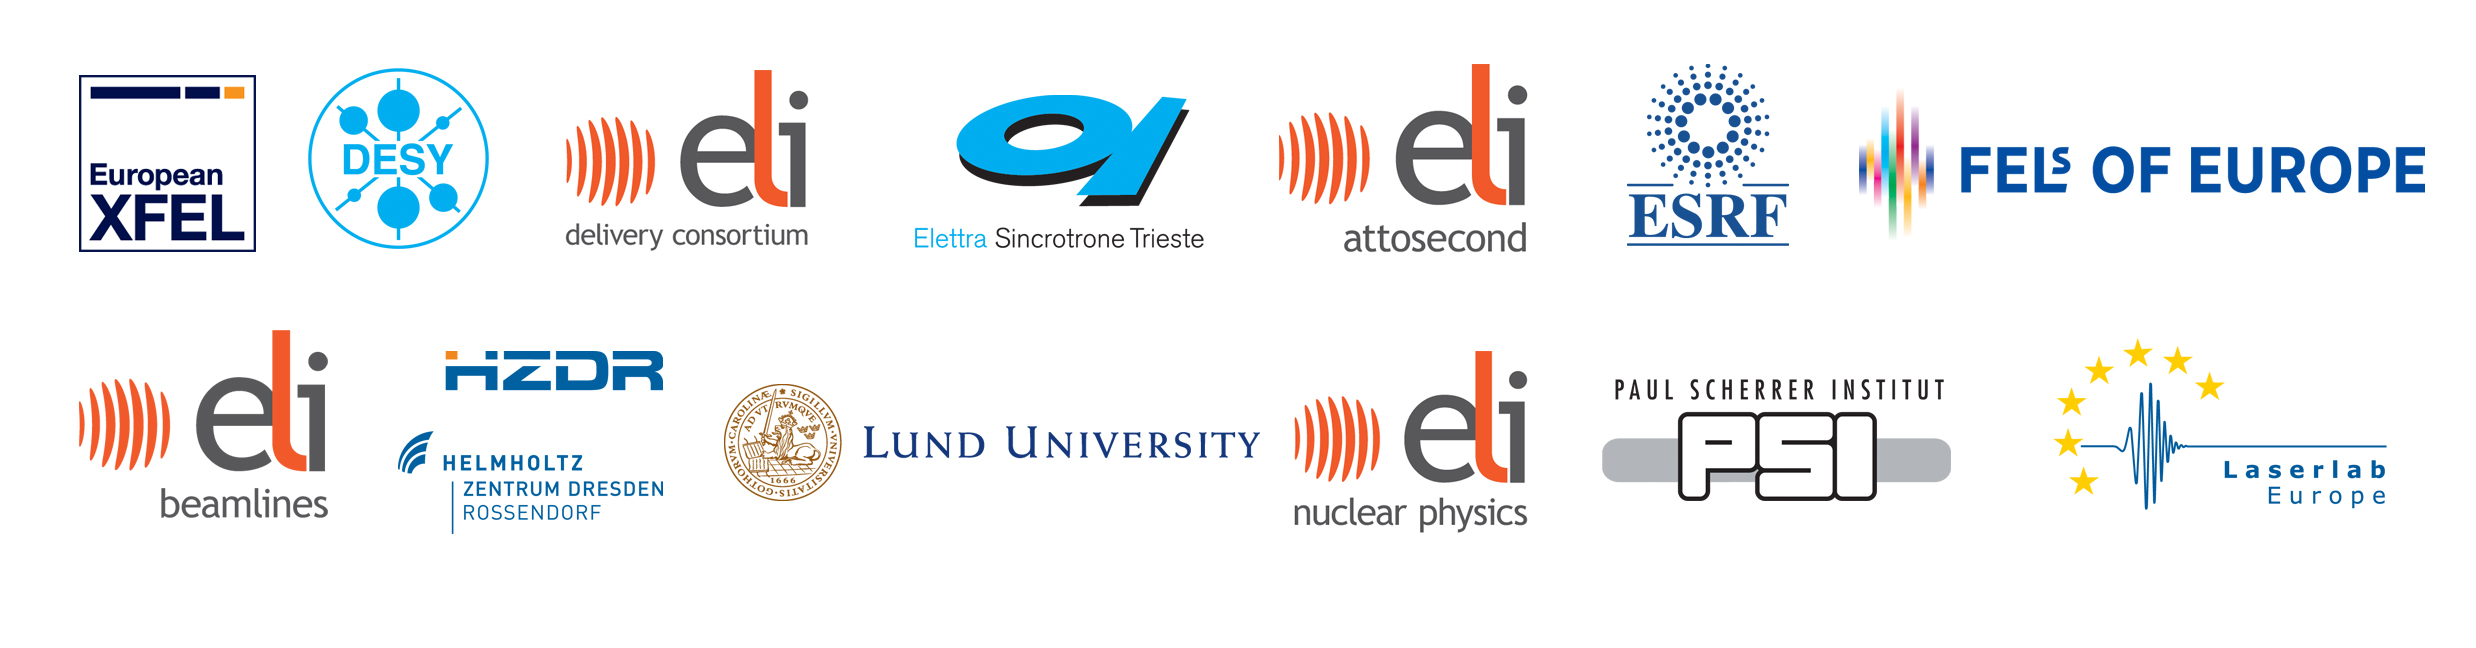
\includegraphics[width=0.91\textwidth]{figures/PartnerLogos_2017}
}
\normalfont
\end{titlepage}
\makeatother

%\tableofcontents

\section{Outline}
%
As first applications of our simulation software suite \textit{simex\_platform}
\cite{simex_github, Fortmann-Grote2017a, EUCALL_SIMEX_D4.3}, we have employed the simulation capabilities of
\textit{simex\_platform} \cite{simex_github} to simulate two photon experiments:
\begin{enumerate}
  \item Coherent diffraction from high--power laser excited optically thin and
    thick plasmas (plasma sample)
  \item Single particle imaging at the European XFEL (non--plasma sample)
\end{enumerate}
%
In addition, we also report on the integration of detector simulations in
\textit{simex\_platform}.

\section{Plasma sample}
%
In Deliverable Report D4.3~\cite{EUCALL_SIMEX_D4.3}, we present the interoperability of \gls{xfel} and \gls{uhi} laser pulse generation,
interaction with the target, and generation of a \gls{saxs} image using the
scattering code \textit{ParaTAXIS}.

A \gls{pic} simulation provides the time
evolution of the electron density on which the \gls{xfel} photons are scattered. We
assume invariance of the target in propagation direction and simulate the \gls{xfel}
pulse with \num{e12} photons for which the target is optically thin,
see left part of Fig. \ref{fig:scattering}. We further demonstrate
scattering on an optically thick setup by simulating
resonant scattering on the ions of the target. The ion density follows the
electron density as expected for plasma expansion into vacuum\cite{Mora2003},
see right part of Fig. \ref{fig:scattering}.

The signal of the optically thick target is washed out due to
higher scattering probability. In both, the optically thin and the optically
thick case, the
\gls{saxs} pattern well resolves the nanometer--scale grating depth and period, taking
into account the target evolution during the interaction time with the laser
pulse.
%
\begin{figure}[ht]
  \centering
  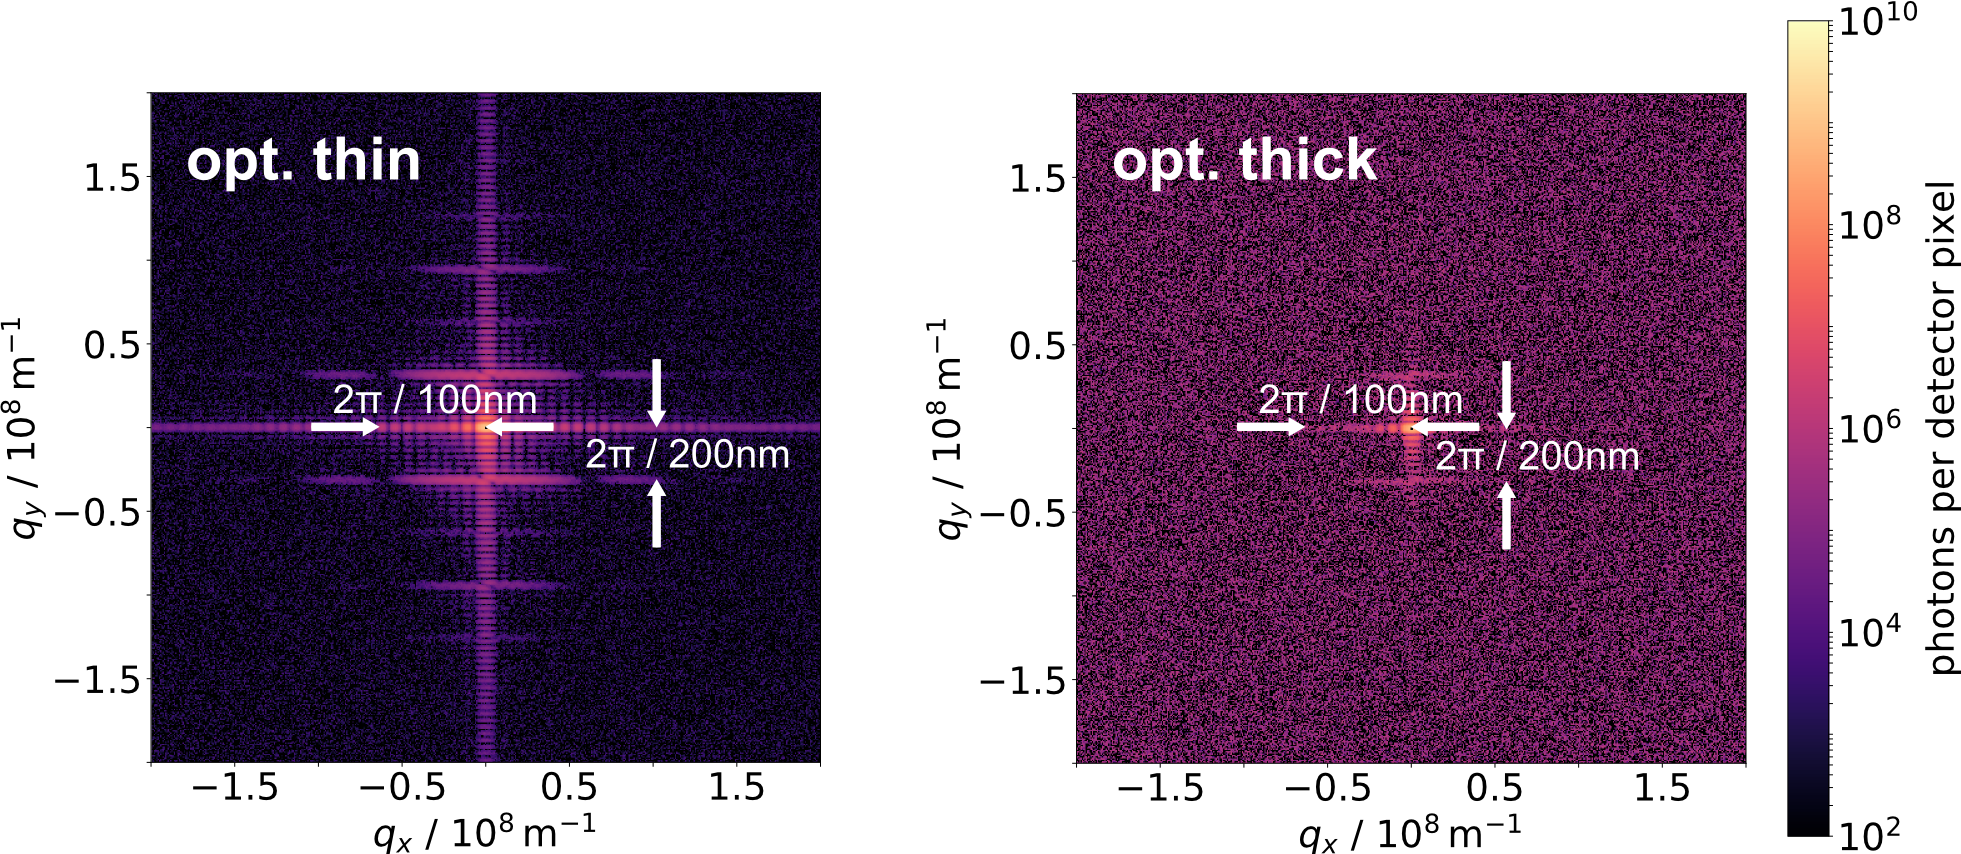
\includegraphics[width=.99\linewidth]{figures/scattering_images_v2.png}
  \caption{
    \textbf{Left:} \textit{ParaTAXIS} \gls{saxs} image for the optically thin target at
    $\SI{1.4}{\metre}$ distance from the target, detector pixel size $a_D =
    \SI{13.5}{\micro\metre}$, X-ray wavelength $\lambda_\mathrm{\gls{xfel}} =
    \SI{1.47}{\angstrom}$ and
    \num{e12} photons in the illuminated area. The vertical separation of scattering
    lines corresponds to the grating period of \SI{200}{\nano\metre}, the horizontal to
    the grating depth of \SI{100}{\nano\metre}.
    \textbf{Right:} \textit{ParaTAXIS} \gls{saxs} image for the optically thick target. Here, the
    scattering cross section was increased by a factor of \num{1000} to account for
  resonant scattering at the ion density. All other parameters remain the same.  }
  \label{fig:scattering}
\end{figure}

All density data from the \gls{pic} simulation as well as the \gls{saxs} patterns are
published on Zenodo together with the data format documentation
\cite{Garten2017.zenodo.885033} in partial fulfillment of EUCALL Milestone M4.3
\cite{EUCALL_SIMEX_M4.3}.

\section{Molecular (non--plasma) sample}
Application of \textit{simex\_platform} to single--particle imaging experiments
at the European X--ray Free Electron Laser (SPB--SFX scientific instrument) has
been published as Ref.~\cite{Fortmann-Grote2017}. It is also the basis for an
online tutorial on the
\href{https://www.github.com/eucall-software/simex_platform/wiki/SimEx-Tutorial}{wiki
pages} of \textit{simex\_platform} and it is
discussed in the EUCALL Milestone M4.2~\cite{EUCALL_SIMEX_M4.2} (First example
simulation).
The datasets for coherent diffraction from the protein 2NIP are deposited on
the \href{https://www.zenodo.org/communities/eucall-data}{EUCALL Data
Repository} \cite{Fortmann-Grote2017.zenodo.886087}.

The signal generation for non--plasma samples happens in two steps: First, the
photon--matter interaction module calculates for each time step of the
simulation the atomic positions and the atomic form factors for each
atom in the sample in the field of the x--ray laser. The effect of radiation
damage can be switched on or off in the simulation. In the latter case, the
atoms remain on their initial positions and the form factors correspond to the
atomic ground states.
This information is then
taken in the second step to calculate the scattered intensity as a function of
time for each pixel in the virtual 2D pixel detector. The software package
\textit{pysingfel} \cite{pysingfel_github} implements the scattering formula
\begin{equation}
  I(\mathbf{q}) = \Omega
  \frac{d\sigma_\mathrm{Th}(\theta)}{d\Omega}\langle I_0\rangle\left|
  \sum_i f_i(\mathbf{q})\mathrm{e}^{i\mathbf{q}\cdot\mathbf{R_i}}\right|^2~,
  \label{eqn:scattering_intensity}
\end{equation}
where $d\sigma_\mathrm{Th}/d\Omega$ is the differential Thomson cross
section,
$\langle I_0\rangle$ is the average pulse intensity, $\Omega$ is the solid
angle spanned by the considered detector pixel.
The wavevector $\mathbf{q}$ depends on the detector geometry (distance
$d$ from the sample) and pixel coordinates ($r_x, r_y$) in the detector plane assumed
to be perpendicular to the beam propagation axis and centered such that the
beam axis intersects the detector plane at its origin:
\begin{equation}
  q=\frac{2\pi}{\lambda}\left(%
  \begin{array}{l}
  \sin(2\theta)\,\cos(\phi)\\
  \sin(2\theta)\,\cos(\phi)\\
  \cos(2\theta)-1
  \end{array}%
  \right) =
  \frac{2\pi}{\lambda}\left(%
  \begin{array}{l}
    \frac{r_x}{\sqrt{r_x^2+r_y^2+d^2}}\\
    \frac{r_y}{\sqrt{r_x^2+r_y^2+d^2}}\\
    \frac{d-\sqrt{r_x^2+r_y^2+d^2}}{\sqrt{r_x^2+r_y^2+d^2}}
  \end{array}%
  \right)~.
  \label{eqn:q_components}
\end{equation}
%$q=\left|\mathbf{q}\right| = 4\pi/\lambda\,\sin(\theta)$.
Here, $2\theta=\arctan\left(\frac{r_x^2+r_y^2}{d}\right)$ is the scattering
angle and $\phi=\arctan\left(\frac{r_y}{r_x}\right)$. In this notation, the
pixel solid angle becomes
$\Omega=4\arcsin\left(a^2/\left[ 4(r_x^2+r_y^2+d^2)+a^2 \right]\right)$, with the pixel
width $a$.

In our simulations, $d=\SI{13}{\centi\metre}$. The
detector is a $512\times512$ array of pixels of side length
$a=\SI{200}{\micro\metre}$ corresponding to one quadrant of a 1 megapixel AGIPD
detector \cite{Allahgholi2015} at the SPB--SFX instrument at European XFEL.

We have applied this simulation toolchain to two cases:
\begin{enumerate}
  \item Diffraction of 5 keV photons from isolated 2NIP molecules and variation
    of the \gls{xfel} pulse duration, published in Ref.~\cite{Fortmann-Grote2017}.
  \item Diffraction of 5 keV photons from hydrated 2NIP molecules and variation
    of the hydration layer thickness, published in
    Ref.~\cite{Fortmann-Grote2017b}.
\end{enumerate}
Fig.~\ref{fig:2nip_diffraction_RD_vs_noRD} shows diffraction patterns from
2NIP with and without radiation damage taken into account in the simulation.
%
\begin{figure}[ht]
  \begin{center}
    \subfloat[no radiation damage]{%
    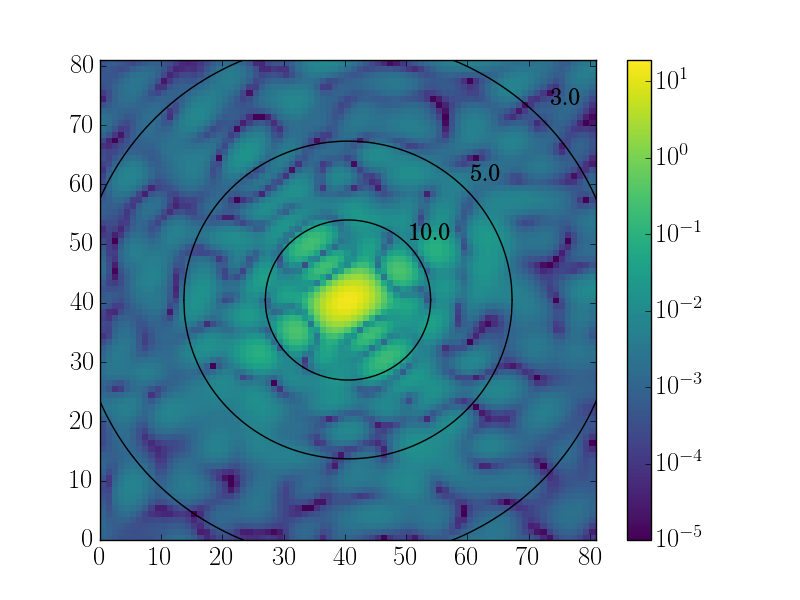
\includegraphics[width=0.4\textwidth,angle=0,clip]{figures/0000283_woRD}%
  }
    \subfloat[with radiation damage]{%
    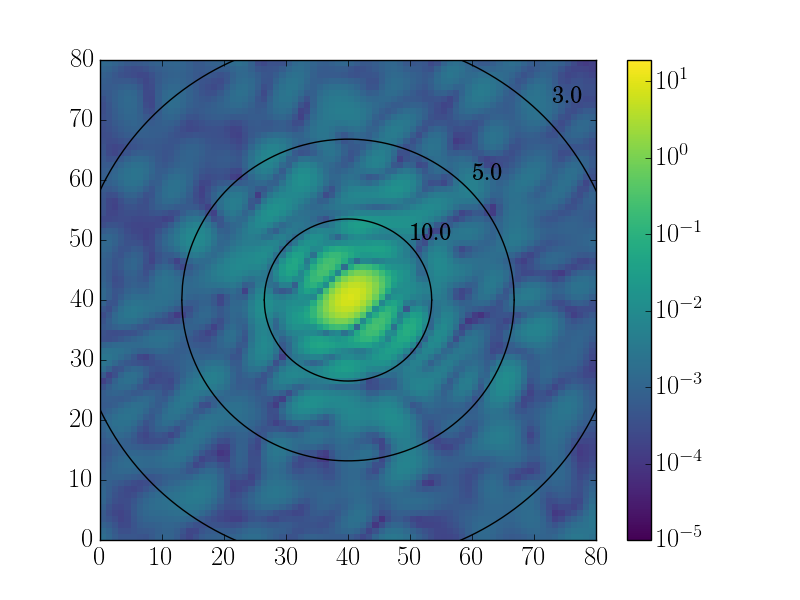
\includegraphics[width=0.4\textwidth,angle=0,clip]{figures/0000283_withRD}%
  }
  \end{center}
  \caption{Diffraction from 2NIP with 5 keV photons without (a) and with (b)
  radiation damage taken into account. Taken from
  Ref.~\cite{Fortmann-Grote2017b}.}
  \label{fig:2nip_diffraction_RD_vs_noRD}
\end{figure}
%
Fig.~\ref{fig:2nip_hydration_layer} shows diffraction from the same molecule for
two different hydration layer thicknesses of \SI{3}{\angstrom} (a) and
\SI{10}{\angstrom} (b), respectively.
%
\begin{figure}[ht]
  \begin{center}
    \subfloat[\SI{3}{\angstrom} hydration layer]{%
    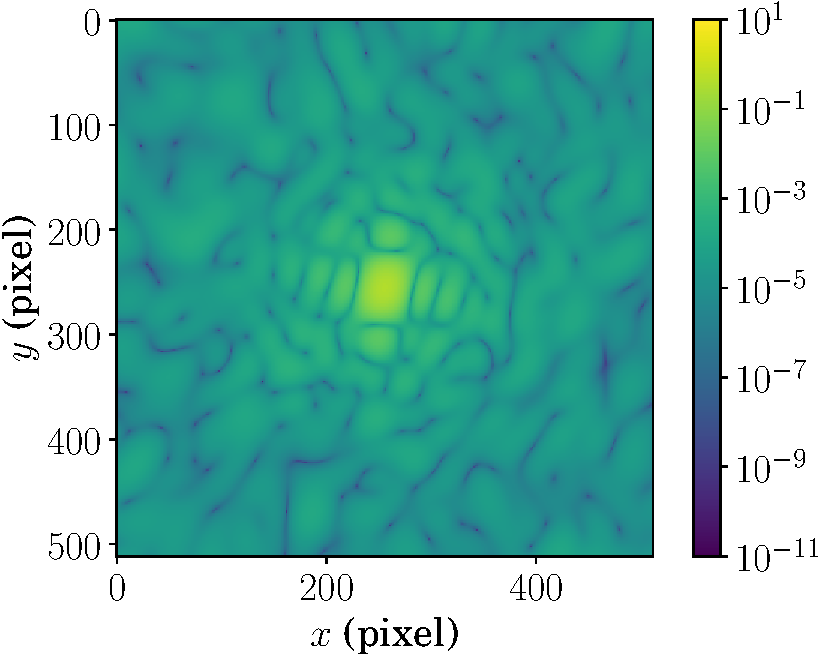
\includegraphics[width=0.4\textwidth,angle=0,clip]{figures/2nip_1diffr_layer3-crop}
  }
    \subfloat[\SI{10}{\angstrom} hydration layer]{%
    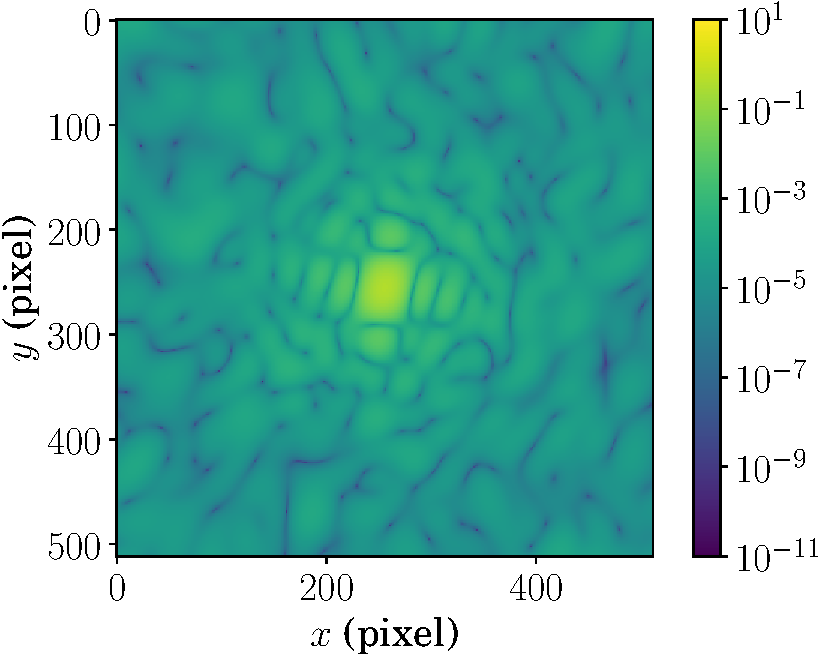
\includegraphics[width=0.4\textwidth,angle=0,clip]{figures/2nip_1diffr_layer3-crop}
  }
  \end{center}
  \caption{Diffraction patterns for 5 keV XFEL photons scattering from a single
    2NIP molecule embedded in a hydration shell of \SI{3}{\angstrom} (a) and
    \SI{10}{\angstrom} (b) thickness.}
  \label{fig:2nip_hydration_layer}
\end{figure}

It can be seen how, qualitatively, the presence of imperfections (radiation
damage or hydration layer) influences the quality of diffraction signals, e.g.
the speckle contrast and noise level.
In both cases, we performed statistical analysis of the simulated diffraction
patterns as a function of the varied parameters pulse duration and hydration
layer thickness, respectively to gain more quantitative insight into the
dependency of diffraction data quality on these effects.

Fig.~\ref{fig:varcoeff} shows the coefficient of variation, a measure of
interpretability of single--particle diffraction patterns \cite{Yoon2016,Fortmann-Grote2017}
for \gls{fel} pulse durations of \SIlist{3;9;30}{\femto\second}. The larger
coefficients of variation found in the  \SI{3}{\femto\second} case indicating
poor data quality is due to the significantly lower photon flux at these
ultra--short pulses. This in turn comes from the intrinsic dependence of pulse
duration on the electron bunch charge \gls{fel}: Highly charged bunches,
producing a high photon flux, experience higher space charge effects and stronger longitudinal dispersion
leading to longer pulse durations.
%
\begin{figure}[ht]
  \begin{center}
    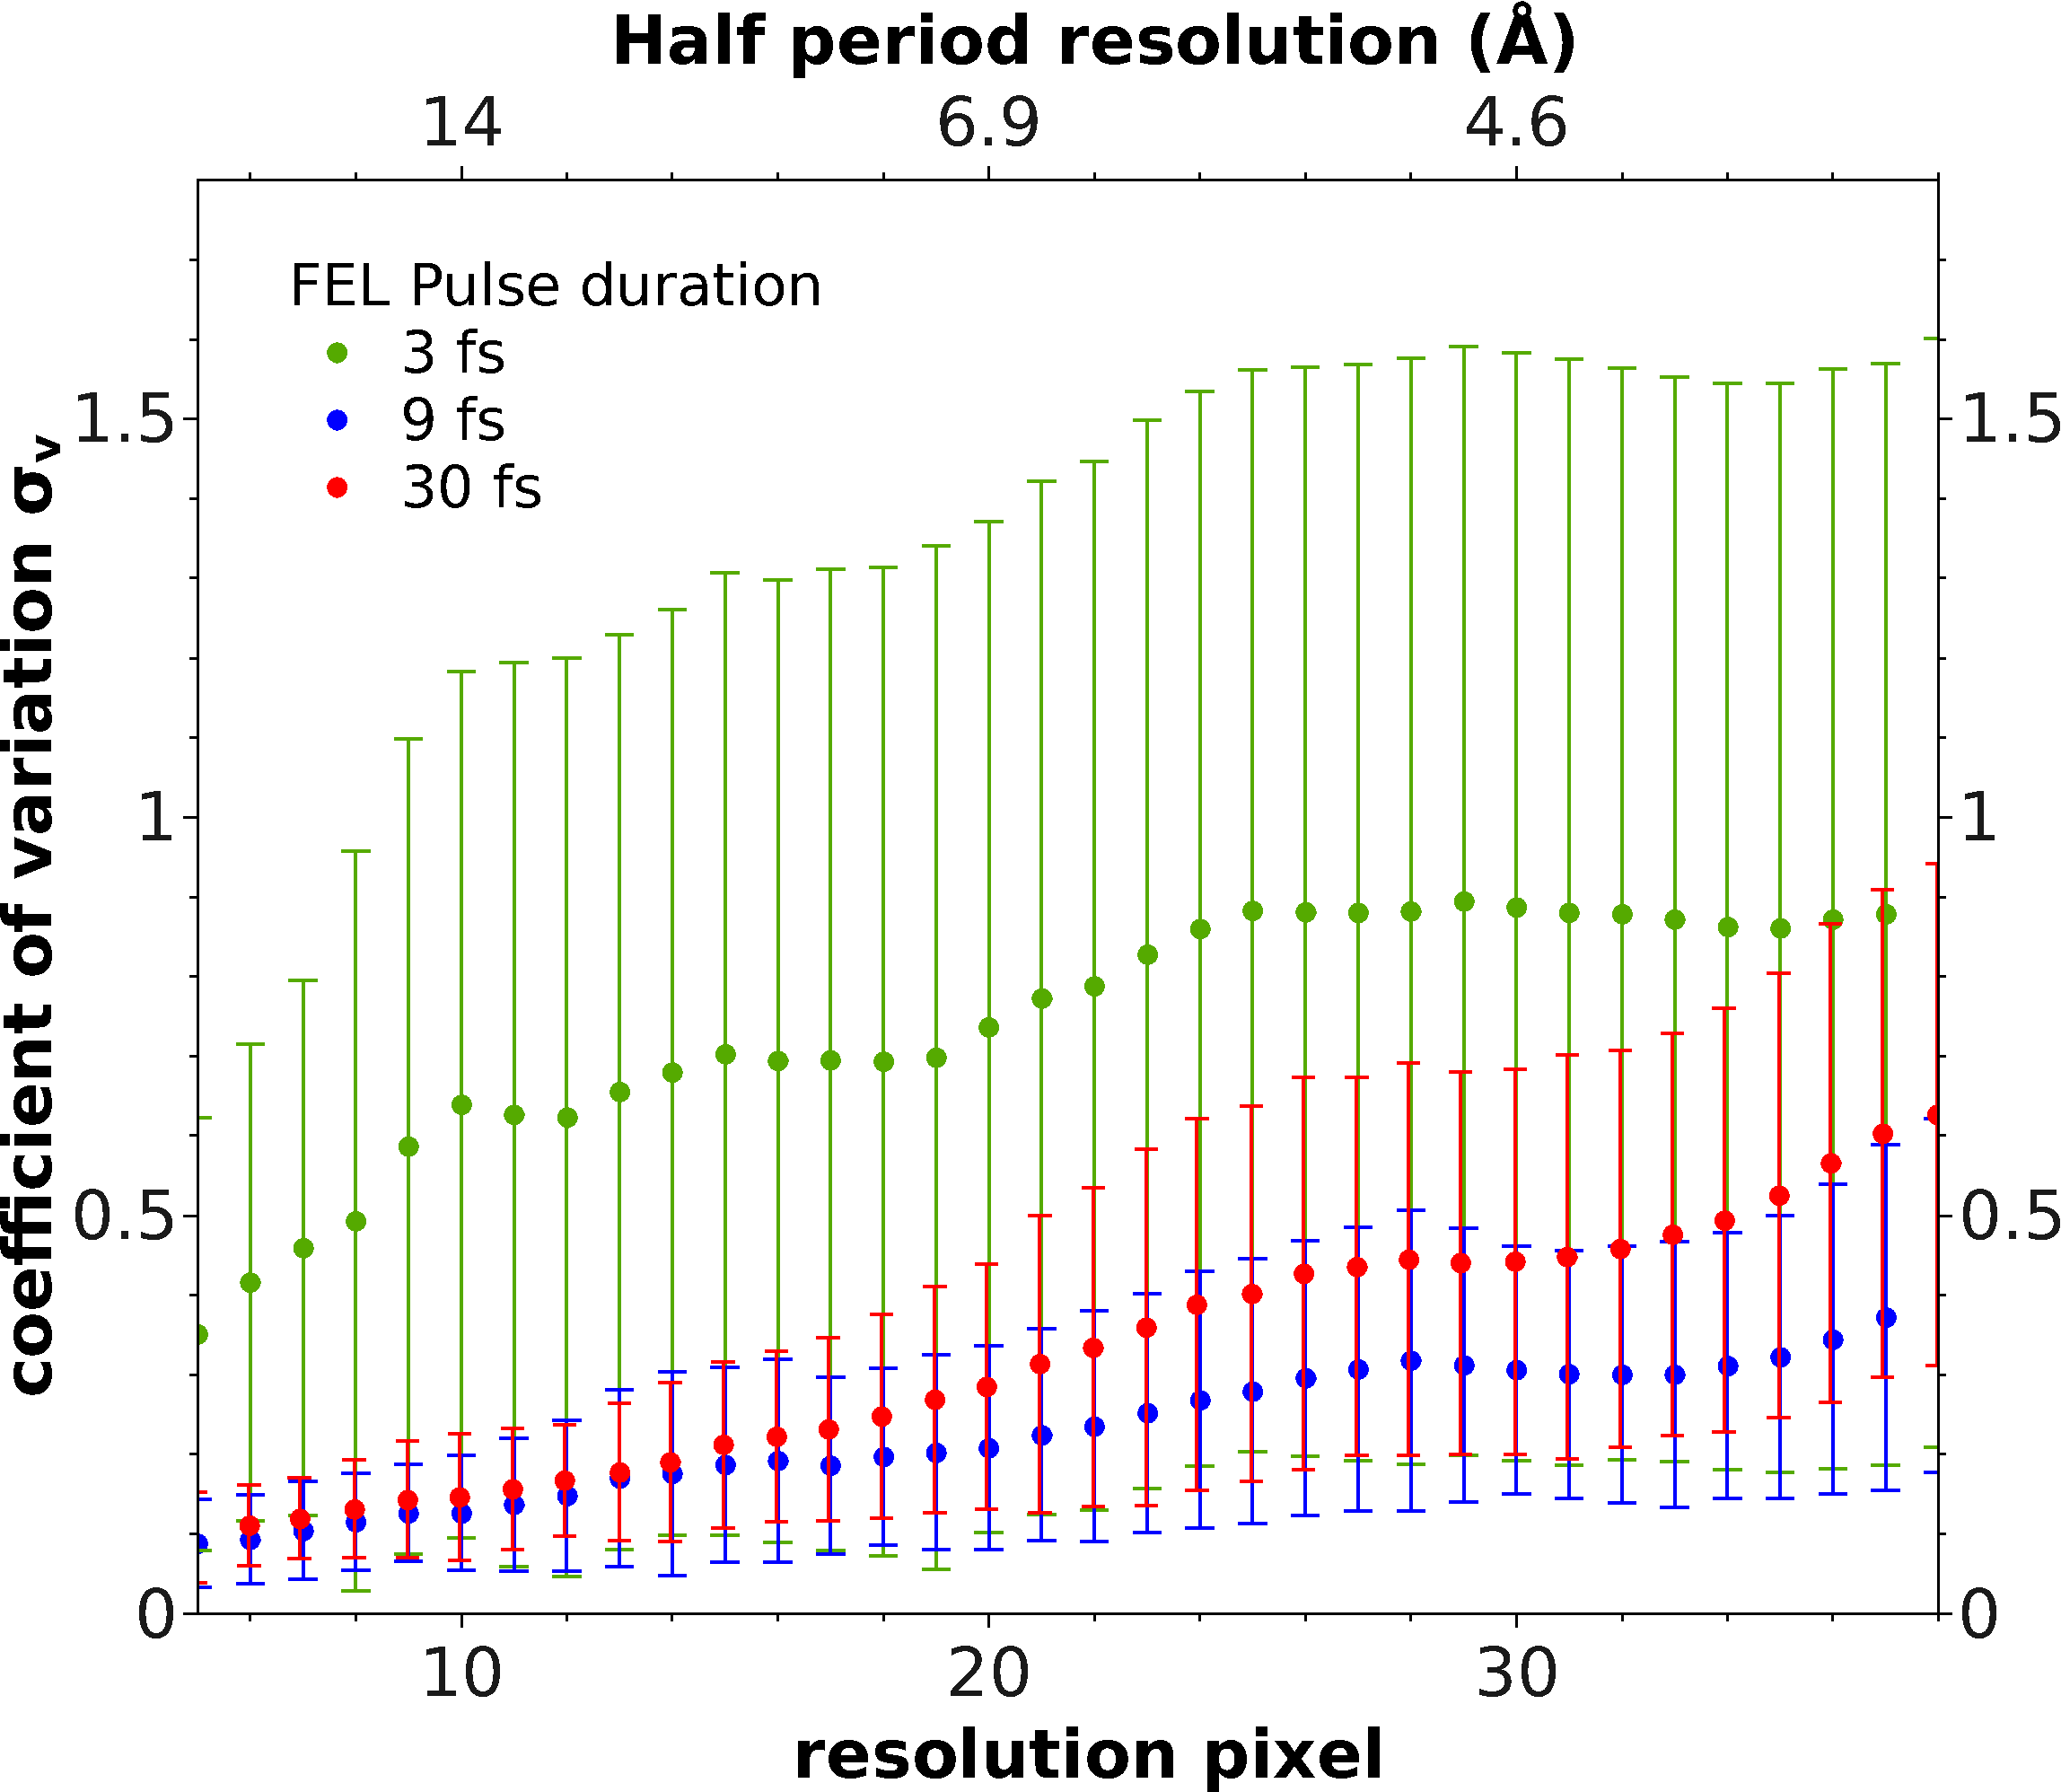
\includegraphics[width=.8\textwidth,angle=0,clip]{figures/varcoeff_3-9-30-crop}
  \end{center}
  \caption{Coefficient of variation obtained from oriented simulated diffraction
  patterns for 2NIP probed by \SI{5}{\kilo\electronvolt} \gls{xfel} pulses of
varying pulse duration and photon flux. Figure taken from Ref.~\cite{Fortmann-Grote2017}.}
  \label{fig:varcoeff}
\end{figure}
%

Fig.~\ref{fig:R_value_hydration} shows the $R$--value for averaged simulated
diffraction patterns as a function of the hydration layer thickness. Radiation
damage has been neglected in these simulations to isolate the effect of the
water presence. $R < 0.2$ indicates good data quality allowing reconstruction of
the 3D electron density at resolution $d=2\pi/q$. Following this argument, the presence of a
\SI{3}{\angstrom} thick hydration layer would allow reconstruction on the level
of a few \si{\angstrom} length scales.
%
\begin{figure}[ht]
  \begin{center}
    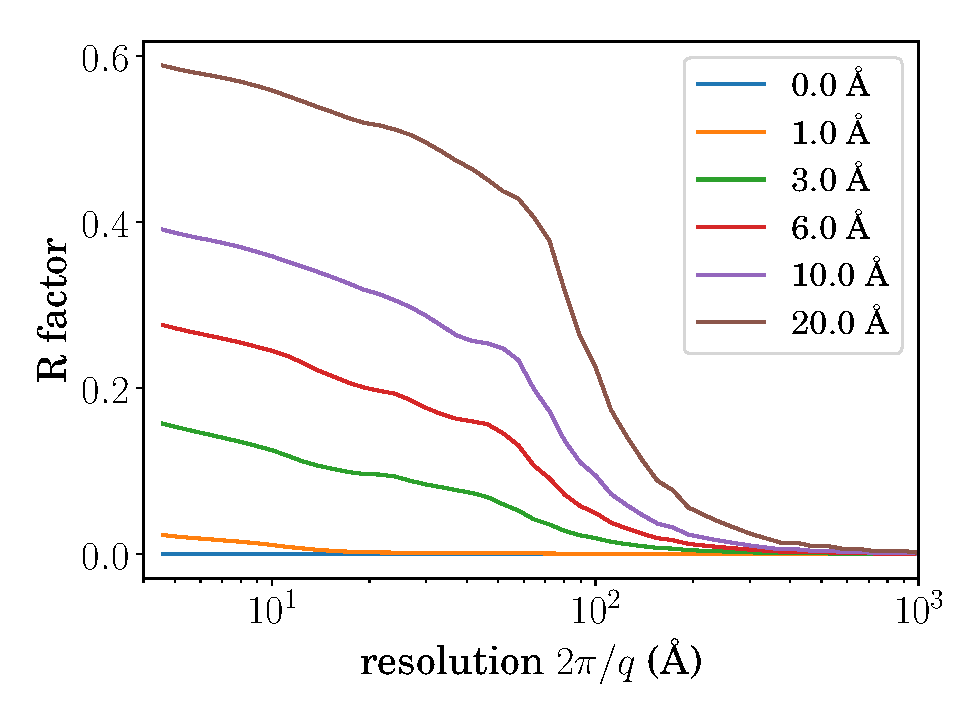
\includegraphics[width=0.8\textwidth,angle=0,clip]{r_factor_vs_layer_thickness}
  \end{center}
  \caption{$R$--value obtained from simulated diffraction patterns for 2NIP
  probed by probed by \SI{5}{\kilo\electronvolt} \gls{xfel} pulses of
  \SI{9}{\femto\second} pulse duration as a function of the hydration layer
  thickness. Figure taken from Ref.~\cite{Fortmann-Grote2017b}}
  \label{fig:R_value_hydration}
\end{figure}

\section{Detector simulations\label{sec:detector_simulations}}
Simulations of measurable signals should not only take into account the
mechanism of x--ray scattering from the sample but also the response of the
detector to the scattered light impinging on the detector surface. So far, these
detector simulations have been missing in \textit{simex\_platform} for various technical reasons as
discussed e.g. in the EUCALL mid term report. These obstacles have now been
overcome. In the following, we present the implementation of detector
simulations in the simulation environment \textit{simex\_platform} followed by a first example simulation.

\subsection{Detector simulation software}
For the purpose of detector simulations, the software packages \texttt{Geant4}
(\url{http://geant4.cern.ch/}) and \textit{X-CSIT}
(\url{https://git.xfel.eu/gitlab/karaboDevices/xcsit}) are utilized that have
already been successfully implemented in the data analysis and control framework
of the European XFEL \textit{karabo}
(\url{https://git.xfel.eu/gitlab/Karabo/Framework}). In contrast to
\textit{karabo}, where all the simulation is performed with devices which are
integrated into the framework processing pipe, \textit{SimEx} is a collection of
classes. Consequently,  installation as well as
maintenance and usage of new components are more convenient in \textit{SimEx}.


Another difference is the programming language:
In contrast to \textit{karabo} and \textit{X-CSIT} which are
written in C++, \textit{SimEx} is written in python. Since \textit{X-CSIT} is
the basis of the simulation also in this project, the interface defined needs to
be made accessible from python. To integrate it into \textit{SimEx} an
additional calculator needs to be written that utilizes the extended functions
from \textit{X-CSIT}. To achieve this, an interface between C++ written
\textit{X-CSIT} and python written \textit{SimEx} source code is designed and
implemented. This includes writing source code in C++ and python as well as
creating a build procedure with \textit{cmake}. Furthermore, an appropriate
documentation and similar coding style like the one used for other
\textit{SimEx} calculators is required.


\subsection{Detector Effects}
\begin{figure}
\centering
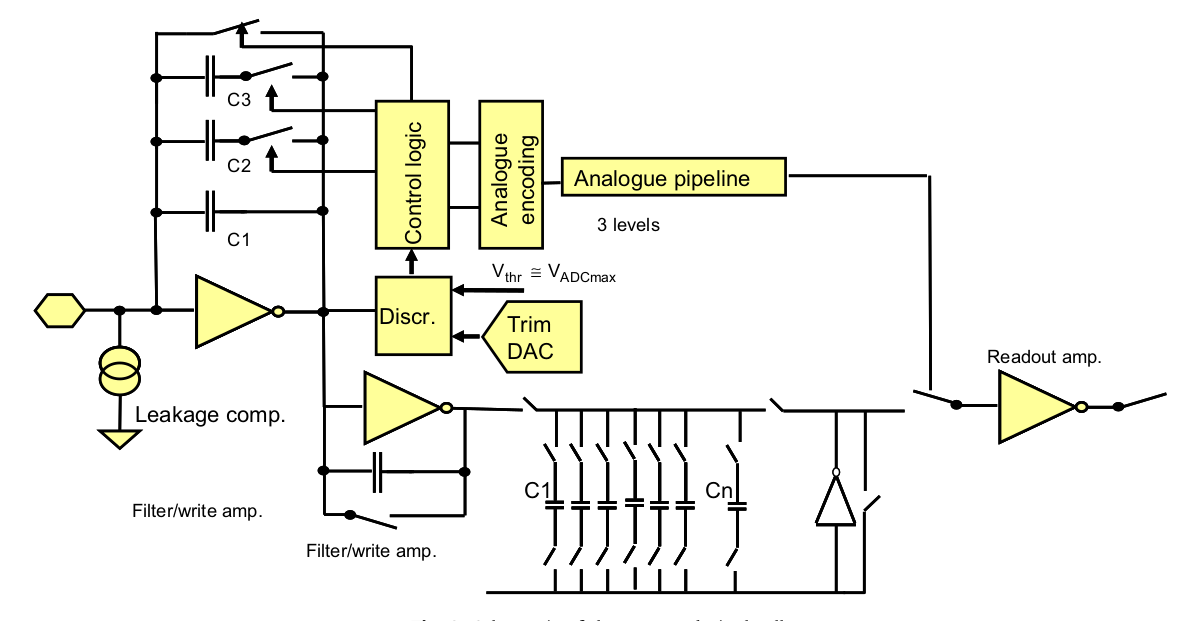
\includegraphics[width=.5\textwidth]{figures/AGIPD.png}
\caption{Application Specific Integrated Circuit of a single pixel of the AGIPD detector with storage pipeline. Source: \cite{henrich2011adaptive}.}
\label{abb. AGIPD}
\end{figure}
Particle detectors are complex electronic devices ranging from
transistors to \glspl{apic}
\cite{potdevin2011analysis} \cite{shi2010challenges}. Due to imperfections in
the material those circuits bear a natural source of fluctuations. Especially,
the influence of leakage currents on operation amplifiers that increase with
radiation intensity can result in increased noise levels
\cite{shi2010challenges}. The resulting noise is often still
smaller than e.g. the statistical fluctuations in the photon number in each
pixel \cite{shi2010challenges}.

Furthermore, leakage currents from another origin are much more serious. Since
the XFEL source produces more images than can be processed in one of its
\SI{600}{\micro\second} pulse trains, the detector needs to store those image values previous
to processing in a pipeline for each pixel (see figure \ref{abb. AGIPD}). After
each of those pulse trains there is a gap of approx. \SI{100}{\milli\second}, where the detector
reads the pixel values of all stored images, digitizes them and store them on a
hard disk. This pipelines consist of capacities and switches that suffer from
leakage currents, as well. This not only affects the output values of intensity
but also the noise level of the readout and digits \cite{shi2010challenges}.

Detectors at European XFEL have to cope with a very complex parameter space.
They have to cover a broad range of energy of many \si{\kilo\electronvolt} for every pixel
independently of each other. Furthermore, the pulse rate of the recording is
quite high. Additionally, they need to be sensible enough to detect single
photons but robust enough not to be destroyed at high intensities. This requires
protection of the electronics leading to additional readout noise
\cite{potdevin2011analysis}. Despite optimizations, detectors have a finite
dynamic range of values, which, once exceeded, leads
cut--off signals \cite{potdevin2011analysis}.

Additionally, there
are also physical effects producing noise. Thermal fluctuations can be reduced
by cooling. However, high intensity radiation can create plasmas in detector
pixels that effect neighbouring pixels due to electron drift
\cite{potdevin2011analysis}. The process is called ``blooming'' and is
taken into account in the charge simulation of this detector simulation project.
Additional information can be found in references: Joy et al. \cite{Joy2015},
R\"uter et al. \cite{Rueter2016}, Shi et al. \cite{shi2010challenges} and Potdevin et al. \cite{potdevin2011analysis}.

Last but not least, the number of photons arriving at a pixel and the number of
charges created from an interacting photon are statistical values. They are
uncertain and follow the Poisson statistics. Together with the blooming this
makes up the most important source for noise. Nevertheless, in many experiments
the noise resulting from a well optimized detector is much less than the
fluctuations in the signal resulting e.g. from optical
elements\cite{potdevin2011analysis}.
%
\subsection{Existing Software}
\subsubsection{Geant4/ X--CSIT}
%
\begin{figure}
  \centering
  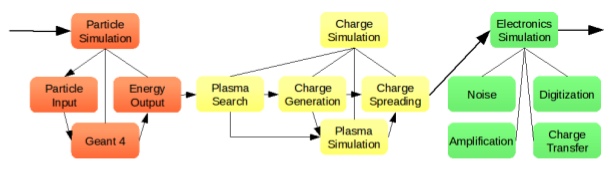
\includegraphics[width=0.6\textwidth]{figures/XCSIT.png}
  \caption{Schema of the different parts of the detector simulation software \textit{X--CSIT}. Source: \cite{Joy2015}.}
  \label{abb. XCSIT}
\end{figure}
%
For the simulation of detectors Joy et al.~\cite{Joy2015} have
created an object oriented software library in the C++ programming language,
called \textit{X--CSIT}\footnote{\textit{X--CSIT} is not free software, hence access
is limited to users who have access to the European
XFEL gitlab repository.}, to simulate the behaviour of 2D semiconductor pixel detectors. Due to
the object orientation not only the initally implmented LPD, AGIPD, DCCS, pnCCD
and FastCCD detectors but also derived detectors can be supported
\cite{Joy2015}. Initially written for being integrated into the \textit{karabo}
framework, the software is universal enough to be stand--alone.

\textit{X--CSIT} consists of three parts \cite{Joy2015} as can be seen in figure
\ref{abb. XCSIT}. The first one, the particle simulation, describes how
photons interact with the active layer of the detector. For this purpose
\textit{X--CSIT} acts as a wrapper of the interaction simulation software
\textit{Geant4} \cite{Joy2015}. \textit{Geant4} covers the physical models of a
broad range of energy ranging from \si{\kilo\electronvolt} to
\si{\tera\electronvolt}~\cite{agostinelli2003geant4}. The
models can handle electromagnetic processes such as the photo electric
effect and fluorescence but also hadronic and optical processes. The standard
processes such as photo electric effect, Compton and Rayleigh scattering, as well
as Auger processes are also included \cite{Joy2015,agostinelli2003geant4}.
For this part \textit{X--CSIT} has the task to
manage the data transfer from and to \textit{Geant4}.
%
\begin{figure}
  \centering
  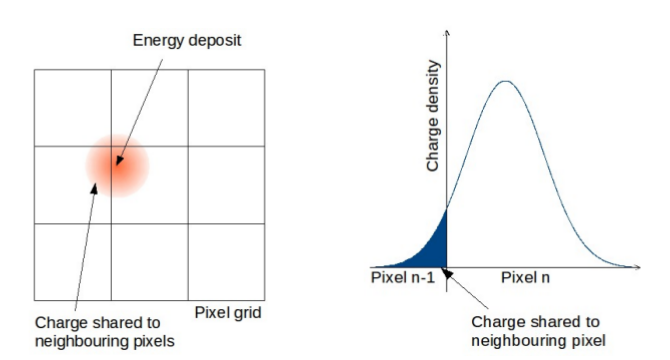
\includegraphics[width=0.6\textwidth]{figures/ChargeSpread.png}
  \caption{Sketch how a charge cloud produced from a single interaction can
    spread to neighbouring pixels. Source: \cite{Joy2015}.}
  \label{abb. Spread}
\end{figure}
%
The second part, the charge simulation, deals with the propagation of the
charges and plasmas created by interactions. Their behaviour is mainly governed
by drift and diffusion of electrons which can be described with a Gaussian
normal distribution (see figure \ref{abb. Spread}) with the following standard
derivation \cite{Joy2015}:
%
\begin{align}
  \sigma_{d} = \sqrt{\frac{2k_{\text{B}} T}{q E} \cdot d}.
\end{align}
%
Here $d$ is the depth in the material, $T$ the temperature, $q$ the drifting
total charge and $E$ the electrical field that pulls the charge to the readout
electronics of the detector.

The last part of \textit{X--CSIT} covers the detector readout electronics.
The electronic simulation simulates the electronic components of the detector
and their behaviour. For this purpose, \textit{X--CSIT} offers modules which are
combined to represent the circuits of the detector \cite{Joy2015}. This
simulation is not included the detector simulations for \textit{simex\_platform} because it
requires a tight connection to, e.g., the calibration software and database for
specific detectors.
%
\subsection{Extending C++ to Python}
Since \textit{X--CSIT} is written in C++ and the calculators of the
\textit{SimEx}\footnote{\textit{SimEx} is the python library inside the simulation
environment \textit{simex\_platform}} are written in python, there is a need of extending C++ classes
to python. To extend the X--CSIT classes to python, we used the
\textit{boost.python} library
(\url{http://www.boost.org/doc/libs/1_65_0/libs/python/doc/html/index.html})
\textit{Boost.python} consits of
header files that need to be added to the C++ implementations. Additionally, in
a BOOST\_PYTHON\_MODULE needs to be defined. This
module creates the equivalent of a python module and needs to define all the
extended classes, their functions as well as their return and input parameters
explicitly \cite{boostpython}. Consequently, \textit{boost.python} can be seen
as a module including abstract types that can be linked to C++ instances as well
as to python instances.

\subsection{Design}
%
\begin{figure}
  \centering
  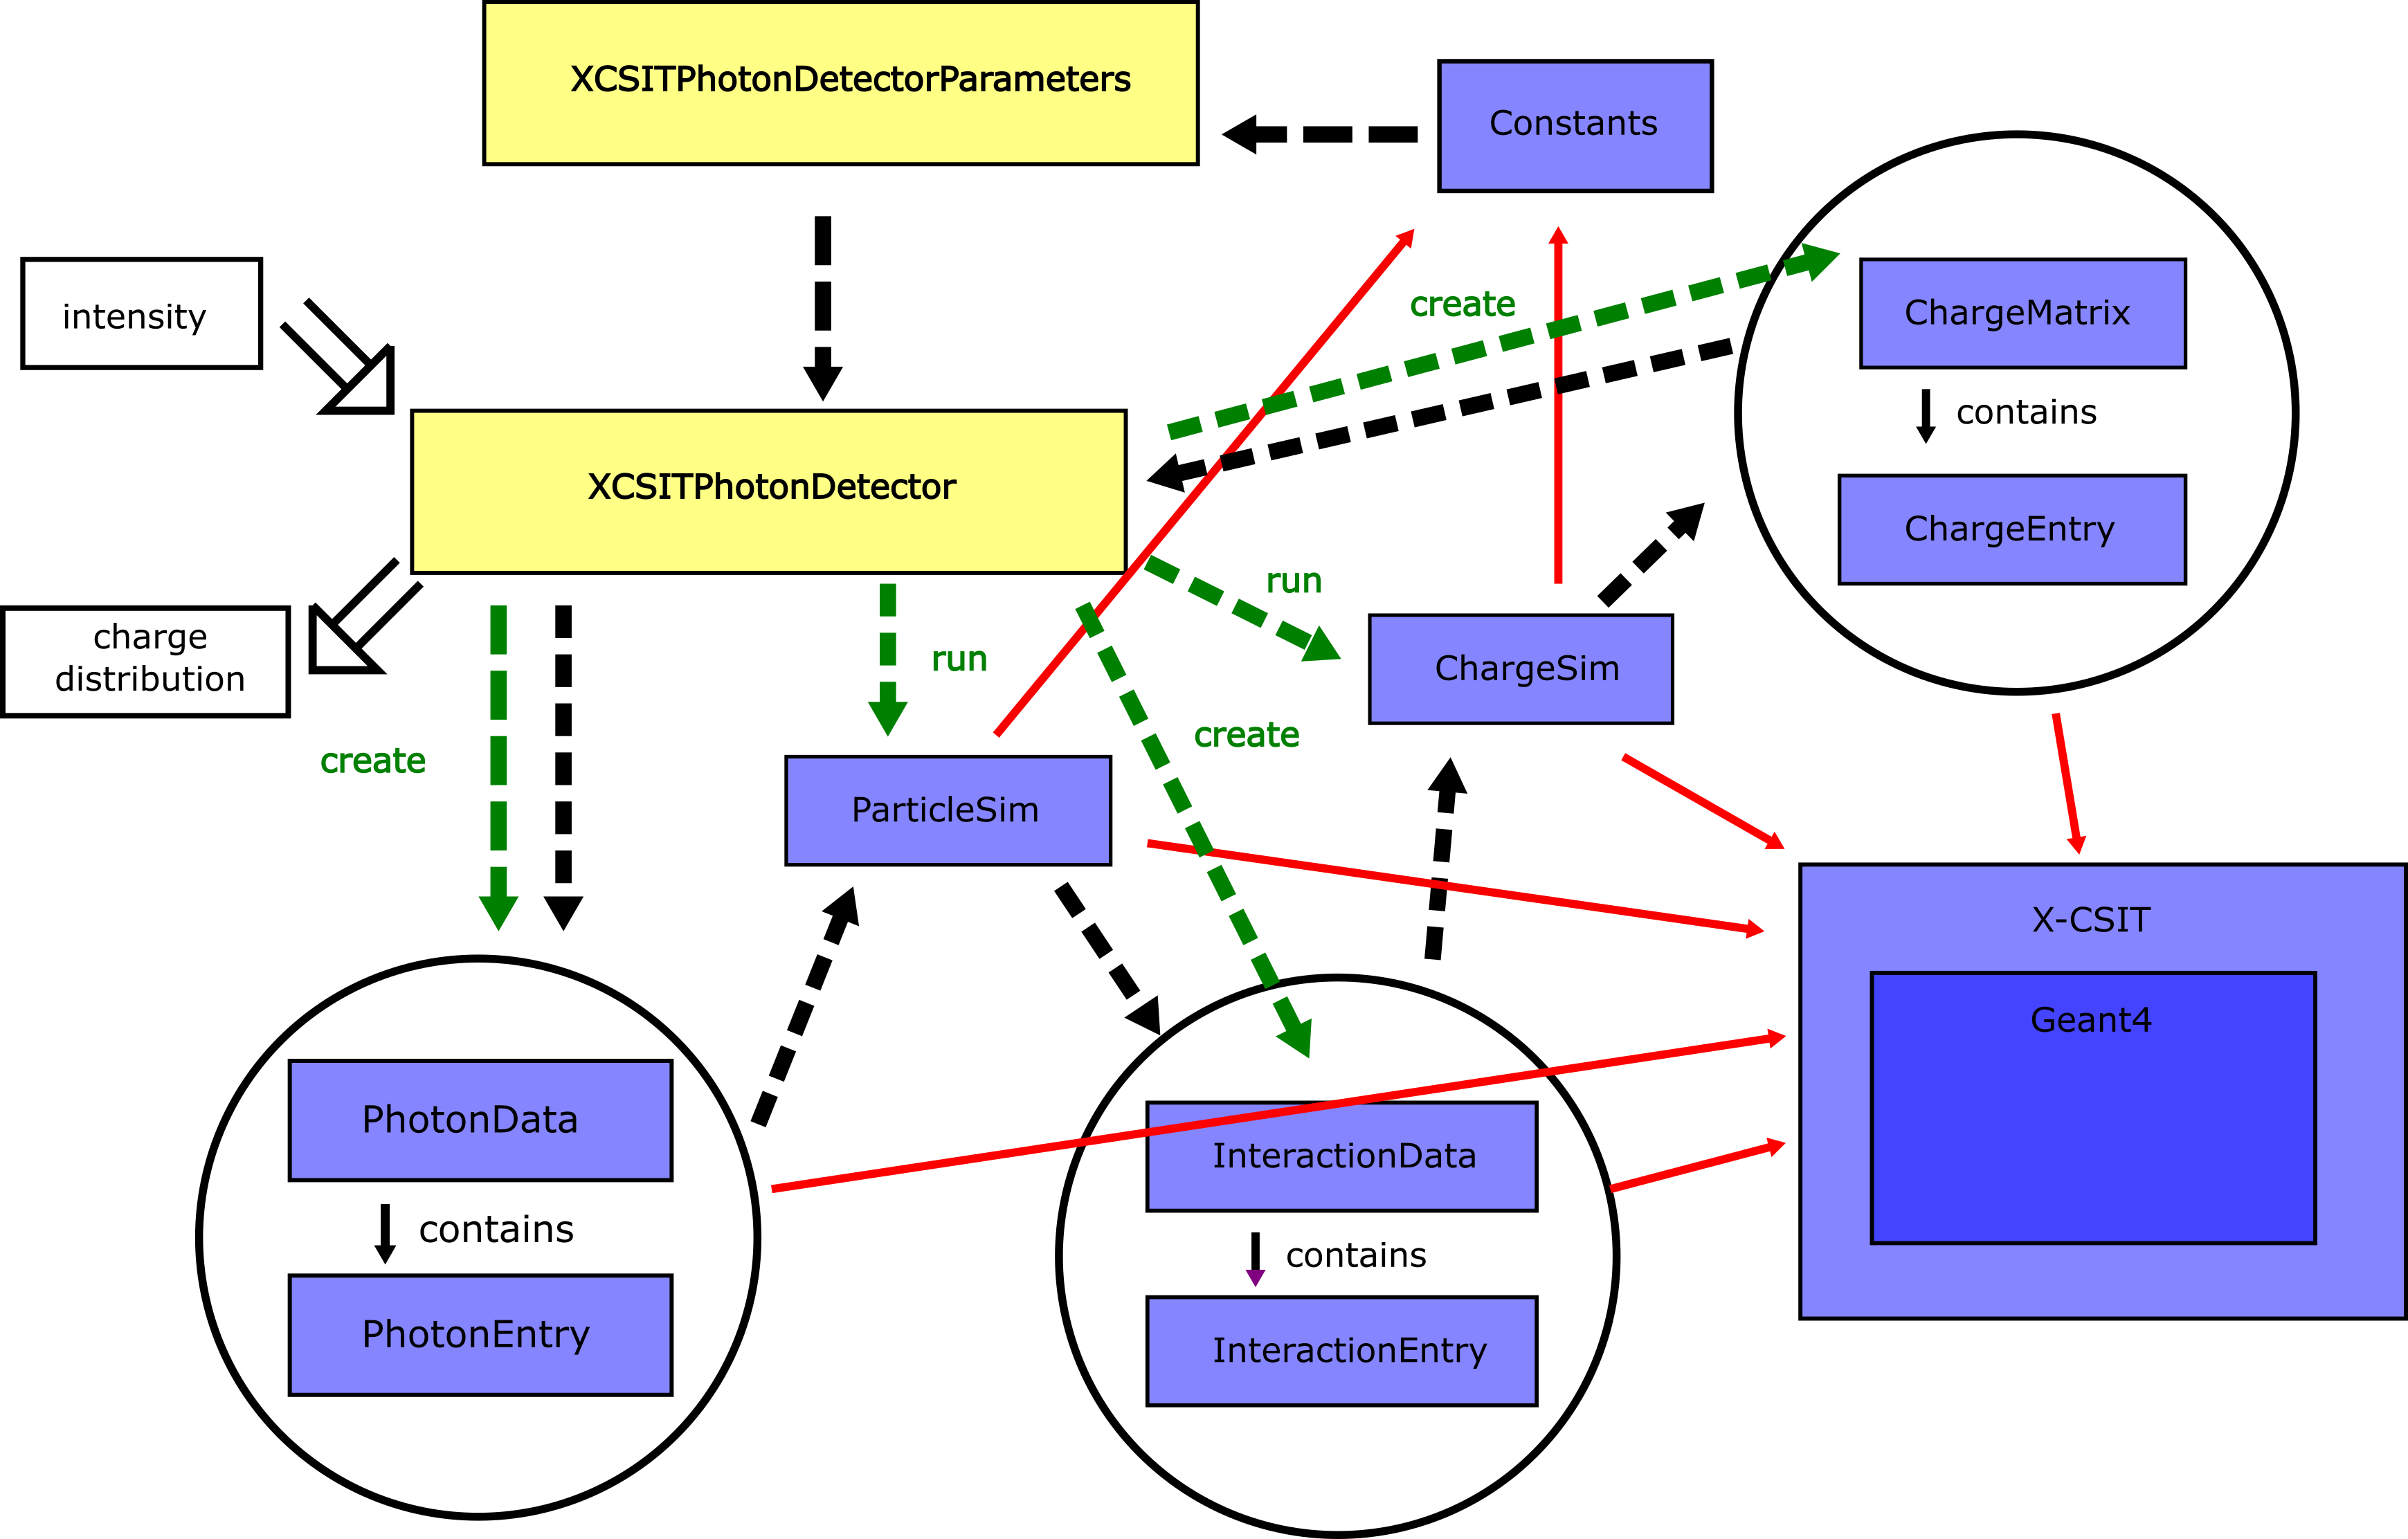
\includegraphics[width=.99\textwidth]{figures/Design.png}
  \caption{Sketch showing the dependencies and inheritance structure of the py\_detector\_interface. Colour code: yellow $\hat{=}$ classes written in python, blue $\hat{=}$ classes written in C++, red arrows $\hat{=}$ inheritance, green arrows $\hat{=}$ manipulation of other instances, black arrows $\hat{=}$ data flow.}
  \label{abb. design}
\end{figure}
Since C++ and python programming languages belong to the object oriented
programming languages, the concept of inheritance and polymorphism are well
suited to achieve the desired extension and integration.
Polymorphism is the key concept for using self written
classes of this design in \textit{X--CSIT}. It allows also to minimize redundant
source code that is always a potential source of error and very difficult to
maintain. However, the required features remain accessible. For this reason, all
the created classes except \textit{Constants} are derived from \textit{X--CSIT}
or \textit{SimEx} base classes and interfaces as can be seen in figure \ref{abb.
design}.

Another important aspect of this design is the design of the python class. In
the end, this is the class that is accessed and used for performing the
simulation. For this reason, it should have control over input and output as
well as control over running the simulation. As can be seen in figure \ref{abb.
design}, the \textit{XCSITPhotonDetector} calculator is given control over each
step of the simulations. This includes creating data containers, initiate and
run the simulations as well as reading the input file and creating the output
file.

Nevertheless, the simulation itself should be triggered from C++ code. One
reason for this is that tunnelling through the \textit{boost.python} layer is
assumed to be slow. Additionally, python code is slower than C++ and there where
additional features needed such as a changed function signature in
\textit{ChargeSim}. Consequently, setting up and running simulations is
programmed in C++ and only calling these functions is extended to python.

Last but not least, the entire project needs to be integrated into
\textit{simex\_platform}. With regard to the source code style and function this can
easily be achieved by applying inheritance. However, one does not want to
compile \textit{X--CSIT} each time you compile also this project. For this
reason, for both \textit{X--CSIT} and py\_detector\_interface \textit{cmake} is
used to compile and link the compiled classes to shared objects. Shared objects
are the Unix equivalents of Windows' dynamical linked libraries (.dll) offering
a comfortable way to release and use applications.

\subsubsection{C++ classes}
There are essentially two groups of C++ classes written for this project. The
first one consists of the input and output containers. They are derived from
abstract interfaces located in \textit{X--CSIT}, which have already an
implementation in \textit{X--CSIT}. The following data containers where implemented
using the abstract \textit{X--CSIT} interfaces: \textit{XPhotonEntry},
\textit{XPhotonData}, \textit{XInteractionData}, \textit{XInteractionEntry},
\textit{XChargeEntry} and \textit{XChargeData}. Due to polymorphism other
\textit{X--CSIT} functions can deal with classes derived from them.

The second group of C++ classes deal with the simulations. There is a simulation
of the photons interacting with the  matter of the detector and a simulation
dealing with the propagation of created charges in the detector. Both
simulations have a parent class in \textit{X--CSIT}. Their task is to behave like
a filter. To run a simulation with the \textit{X--CSIT} parent classes certain
functions with certain formal parameters in their signature have to be called in
a specific sequence. In order to avoid the need to extending all those types
from \textit{X--CSIT} possible to use as these formal parameters the simulation
classes are necessary.

The functions of \textit{ParticleSim} and \textit{ChargeSim} receive strings to
choose which instances of \textit{X--CSIT} need to be instantiated and bound to a
formal parameter of a \textit{X--CSIT} simulation call. Furthermore, this make
addition of e.g. detectors easier because they need to be added to the C++
simulation classes and \textit{Constants} only. There is no need to export them
to python. Currently the following options are included:
%
\begin{table}
  \centering
  \begin{tabular}{c | l }
    \text{category} & \text{options} \\
    \hline
    DetectorType & pnCCD, LPD, AGIPD, AGIPDSPB, CAD \\
    PlasmaSearch & BLANK \\
    PlasmaSim	 & BLANKPLASMA \\
    PointSim	 & FULL, FANO, LUT, BINNING \\
  \end{tabular}
  \caption{This table show the options to choose from when selecting a mode for the simulations.}
  \label{tab. options}
\end{table}
%
Furthermore, the simulation characterisation options specified in table
\ref{tab. options} are needed in various classes. For instance, the \glqq
DetectorType\grqq option is required for both \textit{ParticleSim} and
\textit{ChargeSim}. Additionally, all their constants need to be accessible from
the \\ \textit{XCSITPhotonDetectorParamters} class as well. For this reason, the
constants are stored in an own class. Exploiting the capacities of C++ classes
to inherit from many parent classes, \textit{ParticleSim} and \textit{ChargeSim}
are not just inheriting from their \textit{X--CSIT} parents but also from
\textit{Constants}. In principle, it would also be possible to make \\
\textit{XCSITPhotonDetectorParamters} inherit the constants from
\textit{Constants}. Since this is much more complicated due to the nature of the
attributes of \textit{Constants} (arrays of strings) than adding functions to
\textit{Constants} that return the values, the latter was implemented.

\subsubsection{Python calculators}
Two python classes were written. The first one, \\
\textit{XCSITPhotonDetectorParameters}, implements the abstract python class \\
\textit{AbstractCalculatorParameters}. Its purpose is to gather and check all
the input parameters. If an parameter is set which is not specified in
\textit{Constants} an exception is raised. Nevertheless, instances of this class
are essentially containers with property getter and setter functions. The
properties are the same as the options in table \ref{tab. options}.

The second class is the calculator itself. It implements
\textit{AbstractPhotonDetector} which itself is derived from
\textit{AbstractBaseCalculator}. For this reason, the way the simulation is
performed is already predetermined:
%
\begin{enumerate}
  \item After instantiation python calls immediately the init function. This
    function possesses three formal parameters: a
    \textit{XCSITPhotonDetectorParameters} instance, a variable to store the path
    for the input file and a variable to store the path for the output file. Since
    python variables do not have types, the init function has to check if the
    inserted actual parameters fit with the required instances. Furthermore, init
    deals with incomplete input.
  \item The next method to call is \textit{readH5}.
    Since the input to this calculator is different to the input of
    \textit{ParticleSim} and \textit{ChargeSim}, the data from the hdf5 input file
    has to be translated: The matrix of intensities is read and transformed into
    instances of \textit{PhotonEnty} stored in an instance of \textit{PhotonData}.
    The instances of \textit{PhotonEntry} store for each photon the following
    attributes: energy, normalized vector of flight direction, current position.
    Those values where calculated from the input data by applying geometry.
  %
  \item For running the simulation the \textit{backengine} method has to be called. It consists of two parts:
    %
    \begin{enumerate}
      \item The \textit{PhotonData} instance is passed into \textit{ParticleSim}
        which transfers the container into \textit{XCSIT::XGeant4ParticleSim}
        where interactions of the photons with the detector material are simulated.
        The output container \\ \textit{InteractionData} is also passed to those
        classes. During the simulation it is filled with instances of type
        \textit{InteractionEntry} that contain for each interaction the deposited energy
        in the material at a given site of the detector and the time when that happens
        after start.
      \item The instance of \textit{InteractionData} is handed to the
        instance of \textit{ChargeSim} which transfers it into
        \textit{XCSIT::XPlasmaPointChargeSim} and the \textit{Geant4} \\ classes
        respectively. Since the readout electronics cannot be at the surface of a
        detector an electrical field is applied to pull the created charges in the
        material to the readout electronics. During this propagation charge clouds
        resulting from e.g. plasmas can broaden and effect neighbouring pixels. This
        is simulated in \textit{ChargeSim}. The output is an instance of
        \textit{ChargeMatrix}, where each element, \textit{ChargeEntry},  represents a
        pixel of the detector and each element contains the number of charges recorded
        in that detector pixel. Please note, that the perspective to look at the
        matrix is parallel to the z-axis/ propagation direction of the light.
    \end{enumerate}
    %
  \item Last but not least, the data containers and their content are written to the hdf5 output file at the location specified by the output path.
\end{enumerate}
%
The structure of the input and output file can be found in the wiki of this
project (\url{https://github.com/eucall-software/py_detector_interface/wiki}).
%
\subsection{Application}
%
\begin{figure}
  \centering
  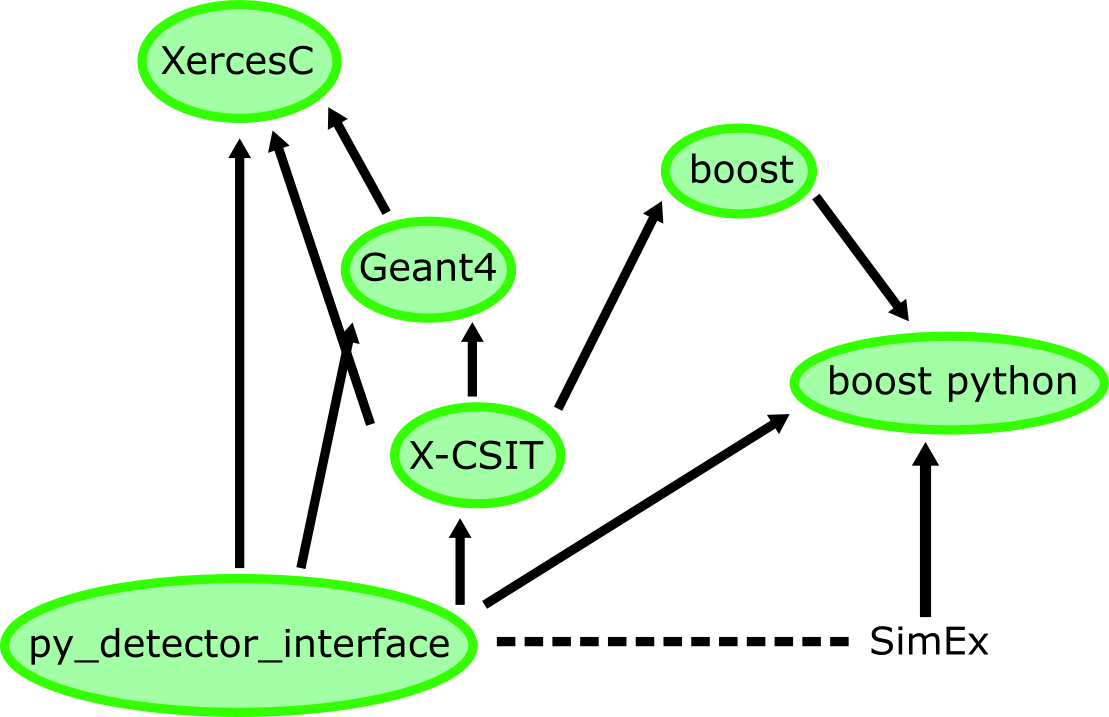
\includegraphics[width=.6\textwidth]{figures/Dependencies.png}
  \caption{Depicted are the dependencies of the py\_detector\_interface project. The green circled names represent shared objects (.so) on Unix operating systems.}\label{abb. dependent}
\end{figure}
%
To test the termination and as a proof of principle the tutorial
(\url{https://github.com/eucall-software/simex_platfrom/wiki/SimEx-Tutorial})
has been used to create a sample diffraction pattern of Nitrogenase Iron protein
from the \textit{Protein Data Base} (see PDB 2NIP \cite{PDB}). The used detector
quadrant of the \glqq AGIPD\grqq  detector has 512 x 512 pixels of
\SI{200}{\micro\metre} x \SI{200}{\micro\metre} size.
All the photons are simulated with an energy of \SI{4.96}{\kilo\electronvolt}
and the detector is \SI{13}{\centi\metre} away from  the origin of diffraction.
To obtain a visible detector response in reasonable compute times,
the scattered intensity was multiplied by a factor \num{e5}.
%
\begin{figure}
  \centering
  \subfloat[Input intensity calculated by the diffraction calculator.]{%
    \centering
    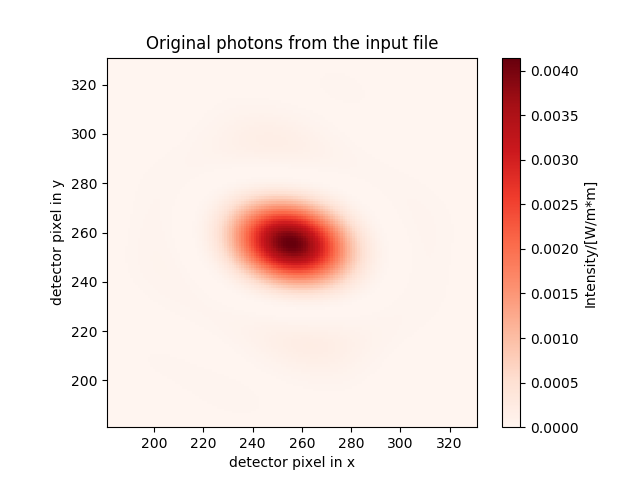
\includegraphics[width=.48\textwidth]{figures/orgphotons.png}
    \label{subabb. diffr in}
  }
  \hfill
  \subfloat[Photonlist created from the the input (see \ref{subabb. diffr in}).]{%
    \centering
    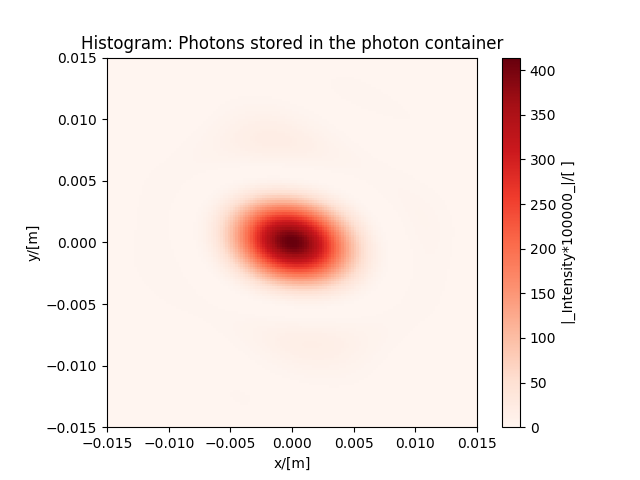
\includegraphics[width=.48\textwidth]{figures/photons.png}
    \label{subabb. photons}
  }\\
  \subfloat[Interactions of the photons with the detector material calculated by X--CSIT and Geant4.]{%
    \centering
    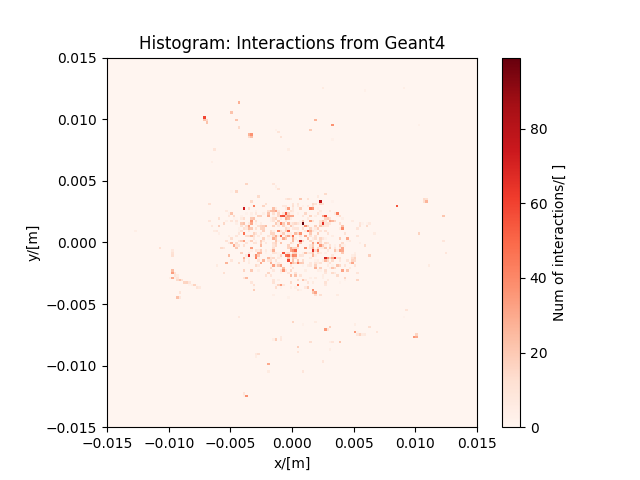
\includegraphics[width=.48\textwidth]{figures/interactions.png}
    \label{subabb. ia}
  }
  \hfill
  \subfloat[Output of the charge propagation simulation.]{%
    \centering
    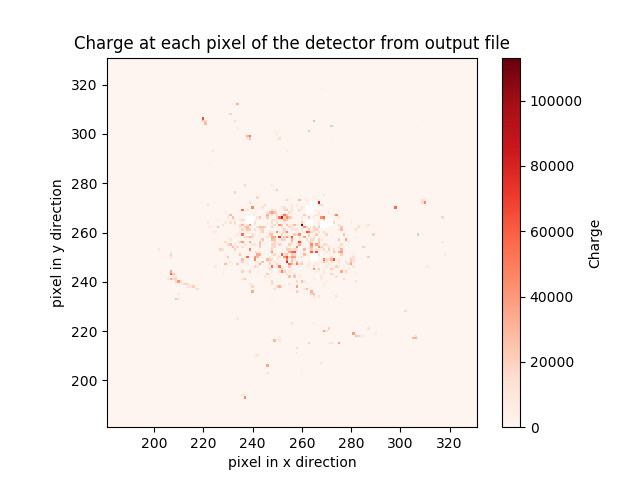
\includegraphics[width=.48\textwidth]{figures/charge.png}
    \label{subabb. charge}
  }
  \caption{This figure shows the state of the data containers at intermediate steps of the simulation. }
  \label{abb. detector sim}
\end{figure}
%
The preliminary results of this study are shown in in Fig.~\ref{abb.  detector sim}).

\subsection{Conclusions}
Detector simulations based on the existing library \textit{X--CSIT} are now part
of \textit{simex\_platform}.
A proof--of--concept simulation demonstrates the workflow. The results will have
to analyzed and the software needs to be profiled and debugged before the
detector simulations can be used in production simulations. This will be among
the upcoming tasks in the SIMEX work package.


\appendix
\section{Deviation from proposal}
As mentioned in the EUCALL mid term report, ELI's contributions to the SIMEX
work package were
re--defined: Within SIMEX, ELI focusses on the development of a simulation
pipeline for \gls{lpa} based coherent light sources. The progress is presented
in the Deliverable Report D4.3 \cite{EUCALL_SIMEX_D4.3}. The task ``signal
generation from plasma samples'' of D4.4  was assigned to HZDR, and the task
``signal generation from non--plasma samples'' was assigned to XFEL.

\FloatBarrier
%%%%%%%%%%%%%%%%%%%%%%%%%%%
\printbibliography[notkeyword=submitted, notkeyword=inpreparation, notkeyword=report, notkeyword=zenodo, title={Journal articles}]
%
\printbibliography[keyword=submitted, title={Submitted articles}]
%
\printbibliography[keyword=inpreparation, title={Articles in preparation}]
%
\printbibliography[keyword=eucall, keyword=report, title={Project reports}]
%
\printbibliography[keyword=zenodo, title={Datasets}]

%%%%%%%%%%%%%%%%%%%%%%%%%%%
\end{document}


